% word limit: 500
\section{Results}

\subsection{Selecting groups of coeval stars}

To explore the relationship between rotation period, \teff\ and age, we
selected groups of stars within different age ranges \citep[where age was
calculated using the][gyrochronology relation]{angus2019}, and calculated the
velocity dispersion: the standard deviation of velocities, \sigmavb, as a
function of effective temperature for each age group.
Since the processes that produce dynamical heating in the galactic disk are
expected to generate Gaussian-distributed velocities, we performed
sigma-clipping on stars in each age and temperature bin, to remove
non-Gaussian outliers.
Ages were calculated using dereddened \gaia\ \gcolor\ color, however
throughout this paper we show rotation periods as a function of {\it effective
temperature}.
We chose to use effective temperatures and not colors in this analysis as it
is the linear quantity and therefore easier to divide into bins of roughly
equal numbers of stars.

\begin{figure}
  \caption{
Top: rotation period vs effective temperature for stars in the \mct\
    catalog.
    The full catalog, with subgiants and visual binaries removed is shown in
    grey, and stars selected to be in different age groups are overlayed in
    color.
    These age groups were selected using the \citet{angus2019} gyrochronology
    relation.
The legend in the center of the figure lists the age range of each group.
    Bottom: velocity dispersion vs effective temperature for each age group.
The color of the line corresponds to the color of the group shown in the top
    panel.
If the gyrochronal model were correct at all ages and the stars in each group
    were the same age across temperatures, the velocity dispersion would be
    constant as a function of \teff.
However, the velocity dispersions of the oldest age groups depend on \teff,
    indicating that the \citet{angus2019} gyrochronology model either
    overpredicts the ages of old M dwarfs or underpredicts the ages of old G
    and K dwarfs.
}
  \centering
    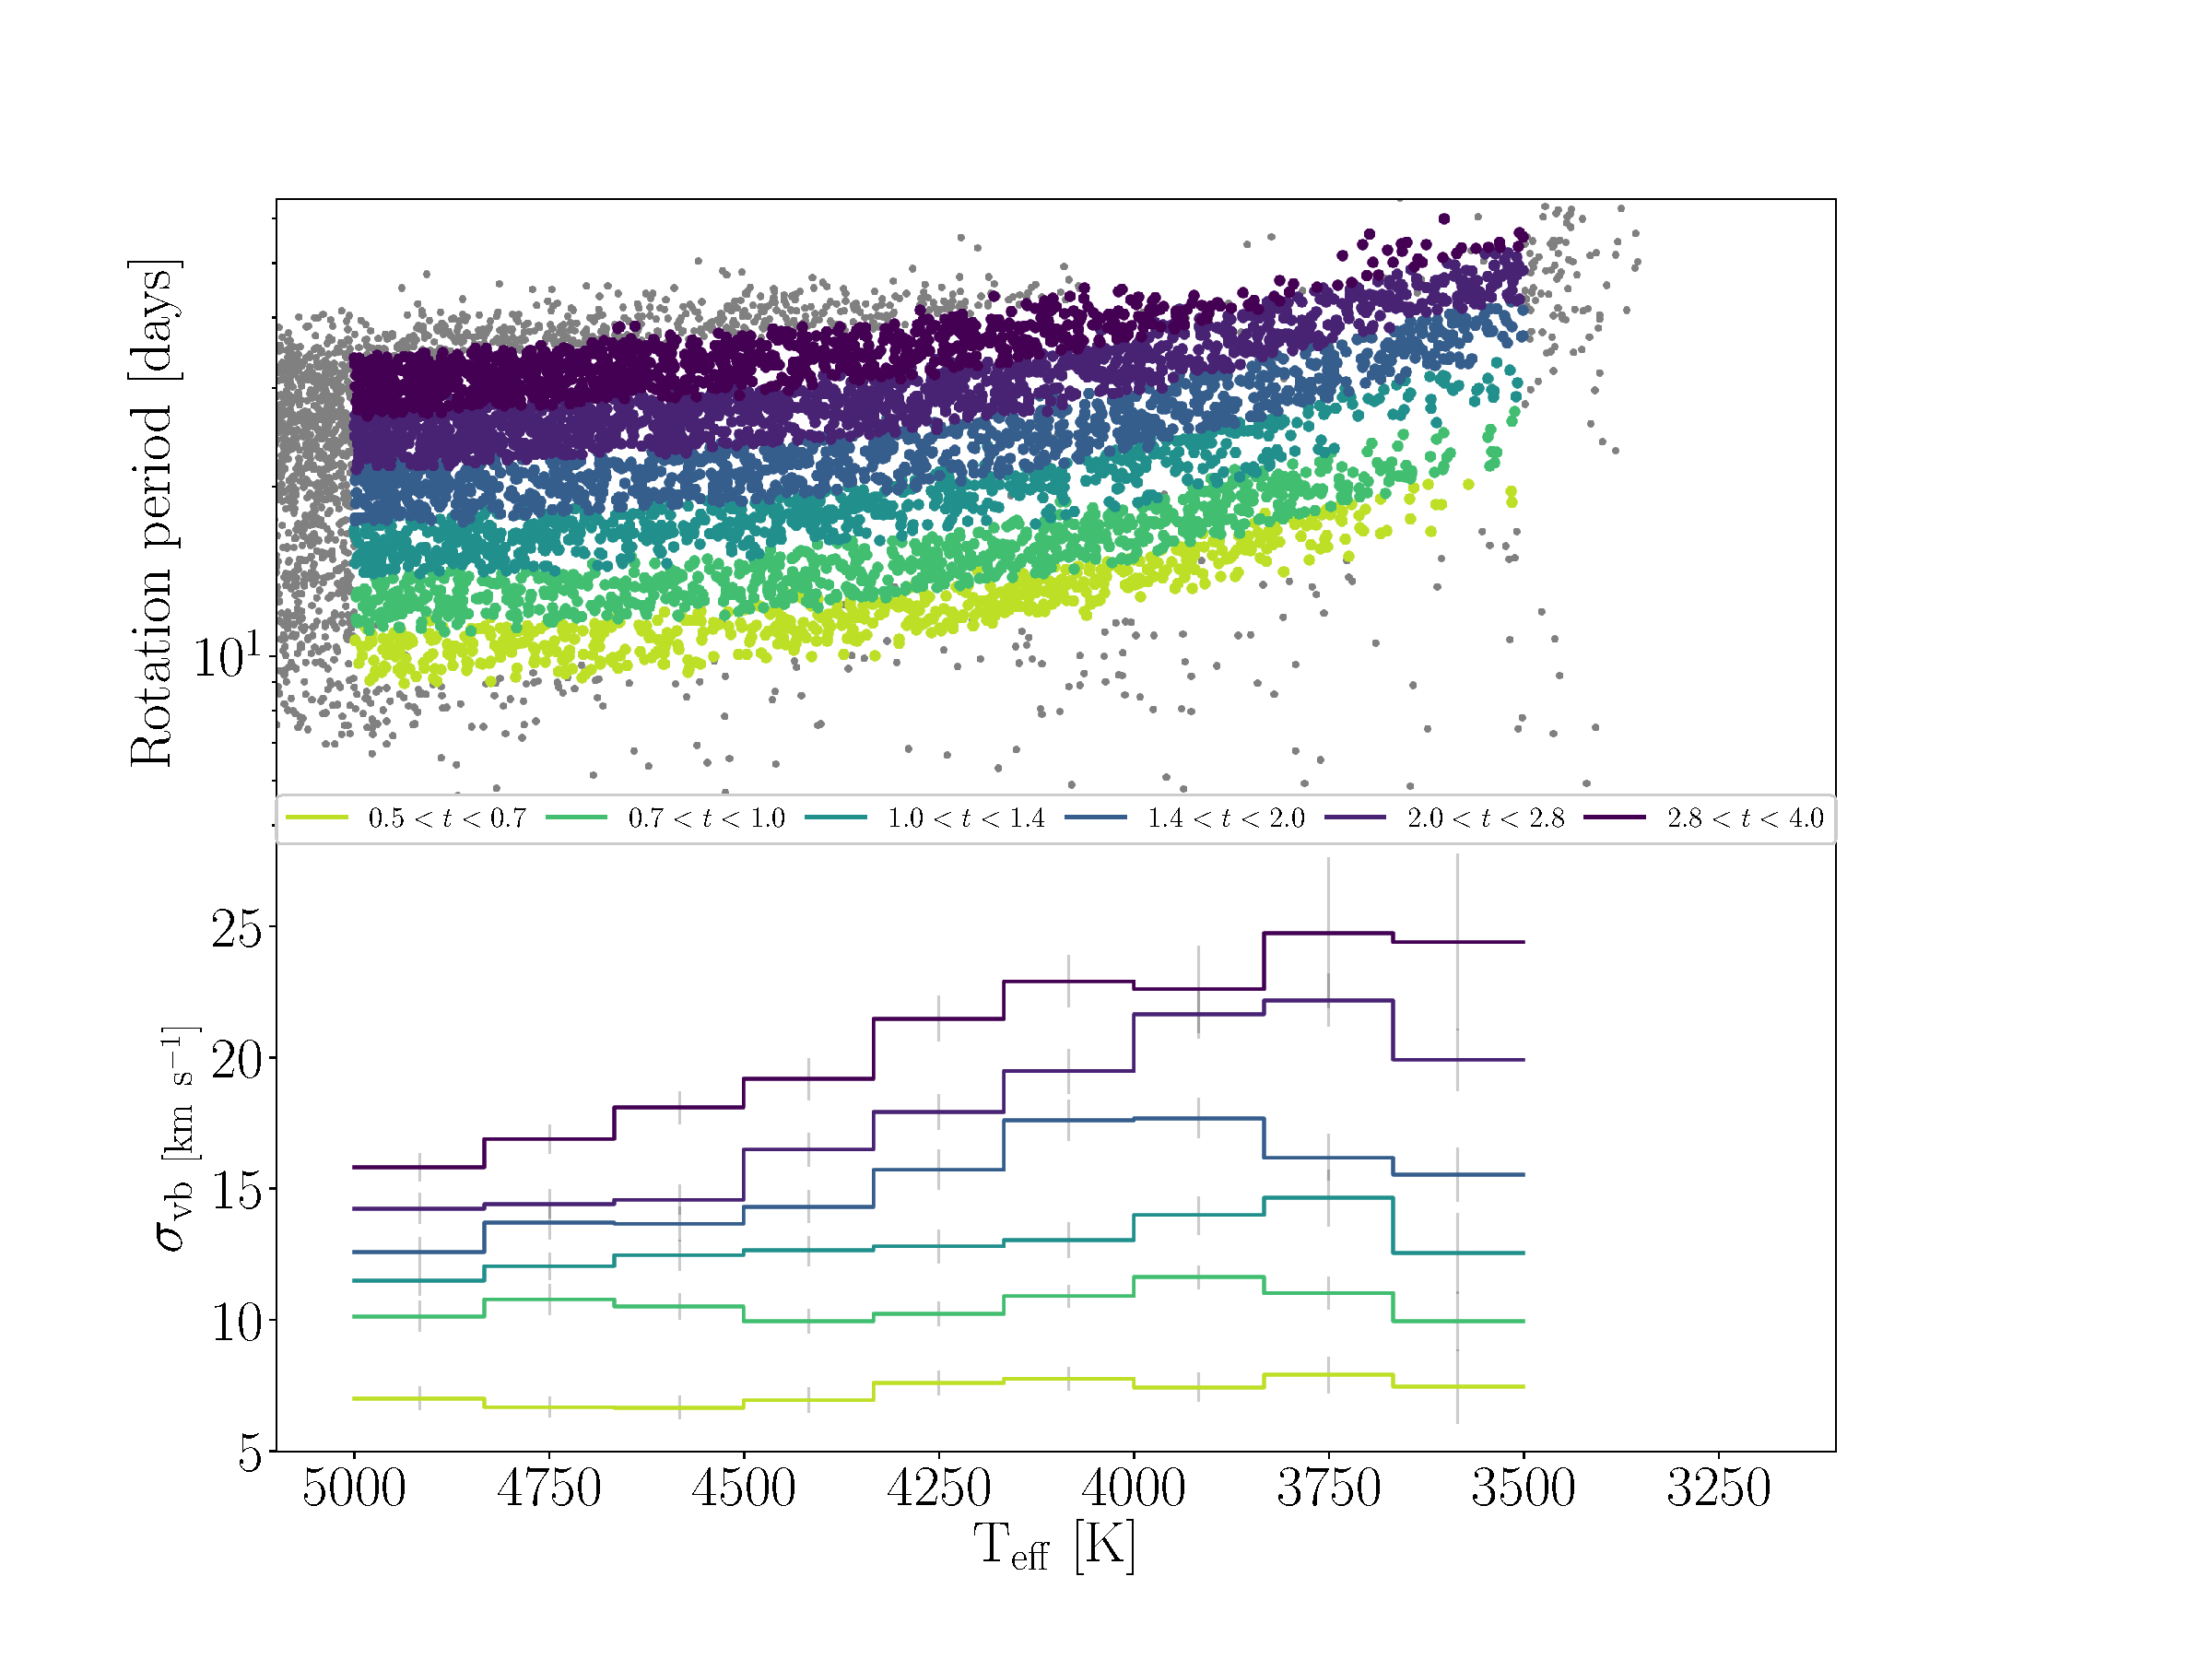
\includegraphics[width=1\textwidth]{age_cut}
\label{fig:age_cut}
\end{figure}
The top panel of figure \ref{fig:age_cut} shows the full \mct\ sample
(excluding visual binaries and subgiants) in grey, with coeval groups shown in
color.
The color of the points corresponds to the age ranges specified in the legend,
which also apply to the lines in the lower panel.
The bottom panel shows the velocity dispersion, \sigmavb\ of each age group,
as a function of effective temperature.
We only included stars within a temperature range of 5000 - 3500 K in our
analysis, as hotter stars are more likely to have stopped magnetic braking
\citep{vansaders2016}, which could bias the results.
M dwarfs were not included in our analysis because such faint stars cannot be
observed at large heights above the plane (because of the low galactic
latitude of the \kepler\ field, stars at high-Z are more distant), which
introduces a mass-dependent velocity bias: cooler populations of stars are
skewed towards lower velocity dispersions.
The coolest temperature bins in figure \ref{fig:age_cut} have low velocity
dispersions, indicating that this effect may already become important at
temperatures lower than $\sim$ 4000 K.

Overall, figure \ref{fig:age_cut} shows that velocity dispersion increases
with gyrochronal age across all temperatures.
However, if the stars in each selected age group had the {\it same} age across
the temperature range, their velocity dispersion would be a constant function
of \teff.
Although the youngest age groups have a relatively constant velocity
dispersions across temperatures, the oldest age groups do not.
This indicates {\it either} that the shape of the period-color relation does
not remain constant over time, \ie\ it flattens out, {\it or} that cool stars
experience more efficient dynamical heating than hot stars.

Mass-dependent dynamical heating could occur because lower-mass stars
experience greater velocity changes when gravitationally perturbed.
However, mass-dependent orbital heating has not yet been unambiguously
observed in the galactic disk because of the strong anti-correlation between
stellar mass and stellar age.
Less massive stars do indeed have larger velocity dispersions, however they
are also older on average \racomment{(citations)}.
This mass-age degeneracy is highly reduced in M dwarfs because their
main-sequence lifetimes are longer than the age of the Universe, however no
evidence for mass-dependent heating has been detected in these low mass stars
\citep{faherty2009}.

The \vb\ AVR is not directly comparable to the \vz\ AVR, so, to draw a
comparison with results from the literature, we calculated a \vz\ AVR for
the subset of 290 stars in our sample with \gaia\ RVs.
We measured an AVR exponent of 0.47 $\pm$ 0.1, which falls within the range of
values (0.45-0.53) reported from measurements of F and G stars in the Solar
neighborhood \citep{holmberg2009, aumer2009, aumer2016}.
It is a little lower than the values of 0.56 $\pm$ 0.14 (for low-z) and 0.51
$\pm$ 0.15 (for high-z stars), calculated using \LAMOST\ \racomment{(LAMOST
citation)} K giants \citep{yu2018}.
K giants are more massive than K dwarfs \racomment{(how much more massive?)},
so this slightly higher value contradicts the mass-dependent heating
hypothesis.
\racomment{Add some words about selection functions...}

To investigate further, we calculated the exponent of the (\vb) AVR for each
temperature bin in figure \ref{fig:age_cut}.
\begin{figure}
  \caption{
The exponent of the AVR as a function of effective temperature.
    The AVR exponent of \citet{holmberg2009}, calculated using a more massive
    sample of stars, is shown as a horizontal dashed line.
}
  \centering
    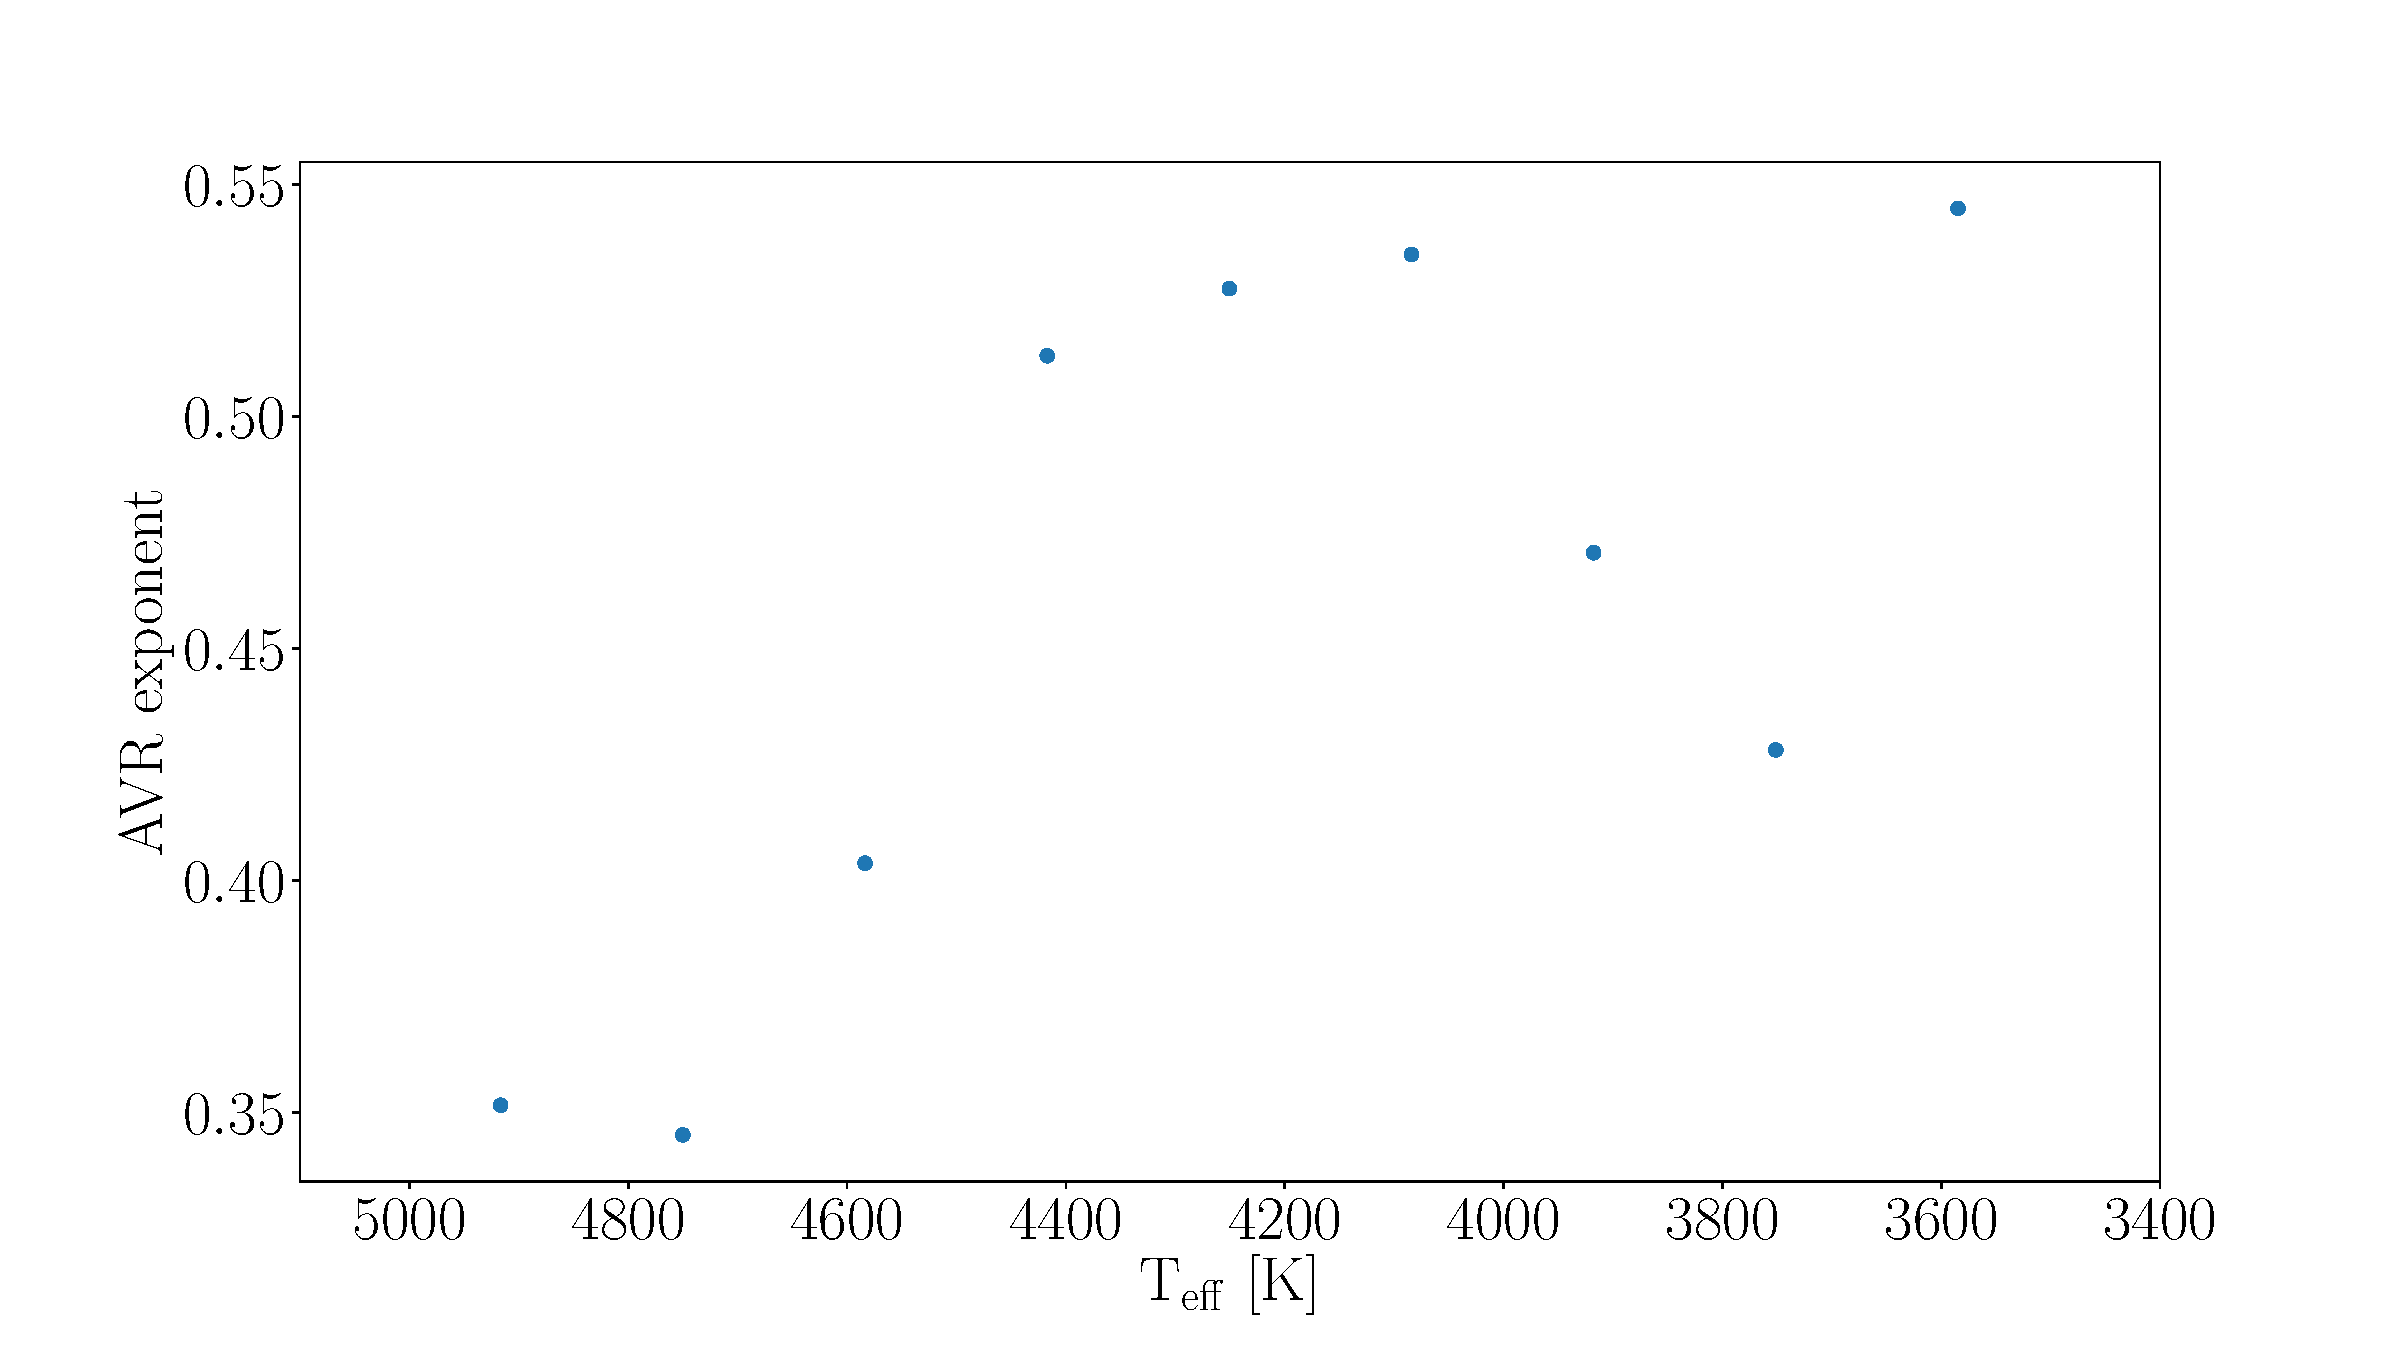
\includegraphics[width=1\textwidth]{AVR_exponent}
\label{fig:AVR_exponent}
\end{figure}

% If mass-dependent heating is strongly affecting our data, the exponent of the
% AVR should increase with decreasing effective temperature, \ie\ the heating
% rate should be greater for lower-mass stars.
% Figure \ref{fig:AVR_exponent} shows the AVR exponent does indeed increase with
% decreasing effective temperature, however, the AVR exponent calculated using
% more massive stars from the Geneva Copenhagen Survey (GCS)
% \citep{holmberg2009} is also shown on this plot as a dashed horizontal line.
% Most GCS stars are F and G type: 1-3 times more massive than the K dwarfs used
% in our study.
% If mass-dependent orbital heating is the main cause the rise in velocity
% dispersion with decreasing \teff\ seen in figure \ref{fig:age_cut}, then the
% AVR exponent of the more massive GCS stars should fall {\it below} the AVR
% exponent for the most massive stars in our sample.
% In other words, the dynamical heating rate should be lowest for the highest
% mass stars and highest for the lowest mass stars.
% % nordstrom2004, jorgensen2005,
% These AVR exponents were calculated with different populations of stars,
% subject to different selection effects, so directly comparing them comes with
% some risk.
% The most important difference is that the GCS AVR is calculated using \vz,
% however our AVRs are calculated using \vb\ since most stars in our sample do
% not have radial velocities.
% The median galactic latitude of these \kepler\ stars is 12.3\degrees, with
% latitudes ranging from 5.5\degrees\ to 21.4\degrees, so \vb\ is a relatively
% close approximation to \vz.
% Only 290 out of the 6820 stars in our sample, plotted in color in figure
% \ref{fig:age_cut}, have \gaia\ radial velocities, however we used the ones
% that do to compare the \vz\ AVR to the \vb\ AVR, across all temperatures
% between 3500 and 5000 K.
% For stars with gyrochronal ages between 0.5 and 4.5 Gyr, we measured a \vz\
% AVR exponent of 0.519 $\pm$ ... and a \vb\ AVR exponent of 0.514 $\pm$... .
% The similarity of these two AVR exponents suggests that directly comparing
% these two quantities {\it may} be a reasonable approach.
% For now, given the large difference between the (\vz) AVR exponent of the GCS
% sample and the (\vb) AVR exponent of the hottest stars in our sample, we
% assume that the increased velocity dispersion at cooler temperatures is mostly
% caused by incorrect age-grouping due to an incorrect period-color relation at
% old ages, and that any mass-dependent heating, while it may contribute at a
% low level to this result, is not the dominant driver.
% However, differentiating the effects of mass-dependent heating and the shape
% of the gyrochronology relations is certainly warranted in a follow-up study.
% }

The consistent velocity dispersion of young stars as a function of temperature
in figure \ref{fig:age_cut} shows that the Praesepe-calibrated gyrochronology
relation accurately predicts the relative ages of {\it young} field stars.
To our knowledge, no gyrochronology relation has never been demonstrated to
correctly predict ages (either relative or absolute) for such cool or such
young field stars.
This is not particularly remarkable however, since these young stars are a
similar age to the Praesepe cluster, which was used to calibrate the
period-color relation.

% Figure \ref{fig:age_comparison} shows the ages of star groups, predicted with
% the \citet{angus2019} gyrochronology relation, compared with the ages of star
% groups, predicted with the \citet{holmberg2009} AVR.
% \citet{holmberg2009} only provide an exponent (0.53), not an intercept, for the
% relation between logarithmic age (in Gyr) and logarithmic, \vz\ velocity
% dispersion (in \kms), so we fit the intercept to the mean \vb\ velocity
% dispersion across all temperatures, of our sample.
% \begin{figure}
%   \caption{
%       Ages predicted by the \citet{holmberg2009} \vz\ AVR, against ages
%     predicted by the \citet{angus2019} gyrochronology relation, for stars in
%     different temperature ranges.
% Points are colored by the effective temperature in the center of the \teff\
% bin.
% The dashed line shows the y=x relation.
% Predicted kinematic ages fan out over gyrochronal time, either because the AVR
%     is temperature-dependent or because the gyrochronology relations have an
%     age-dependent period-color relation.
% }
%   \centering
%     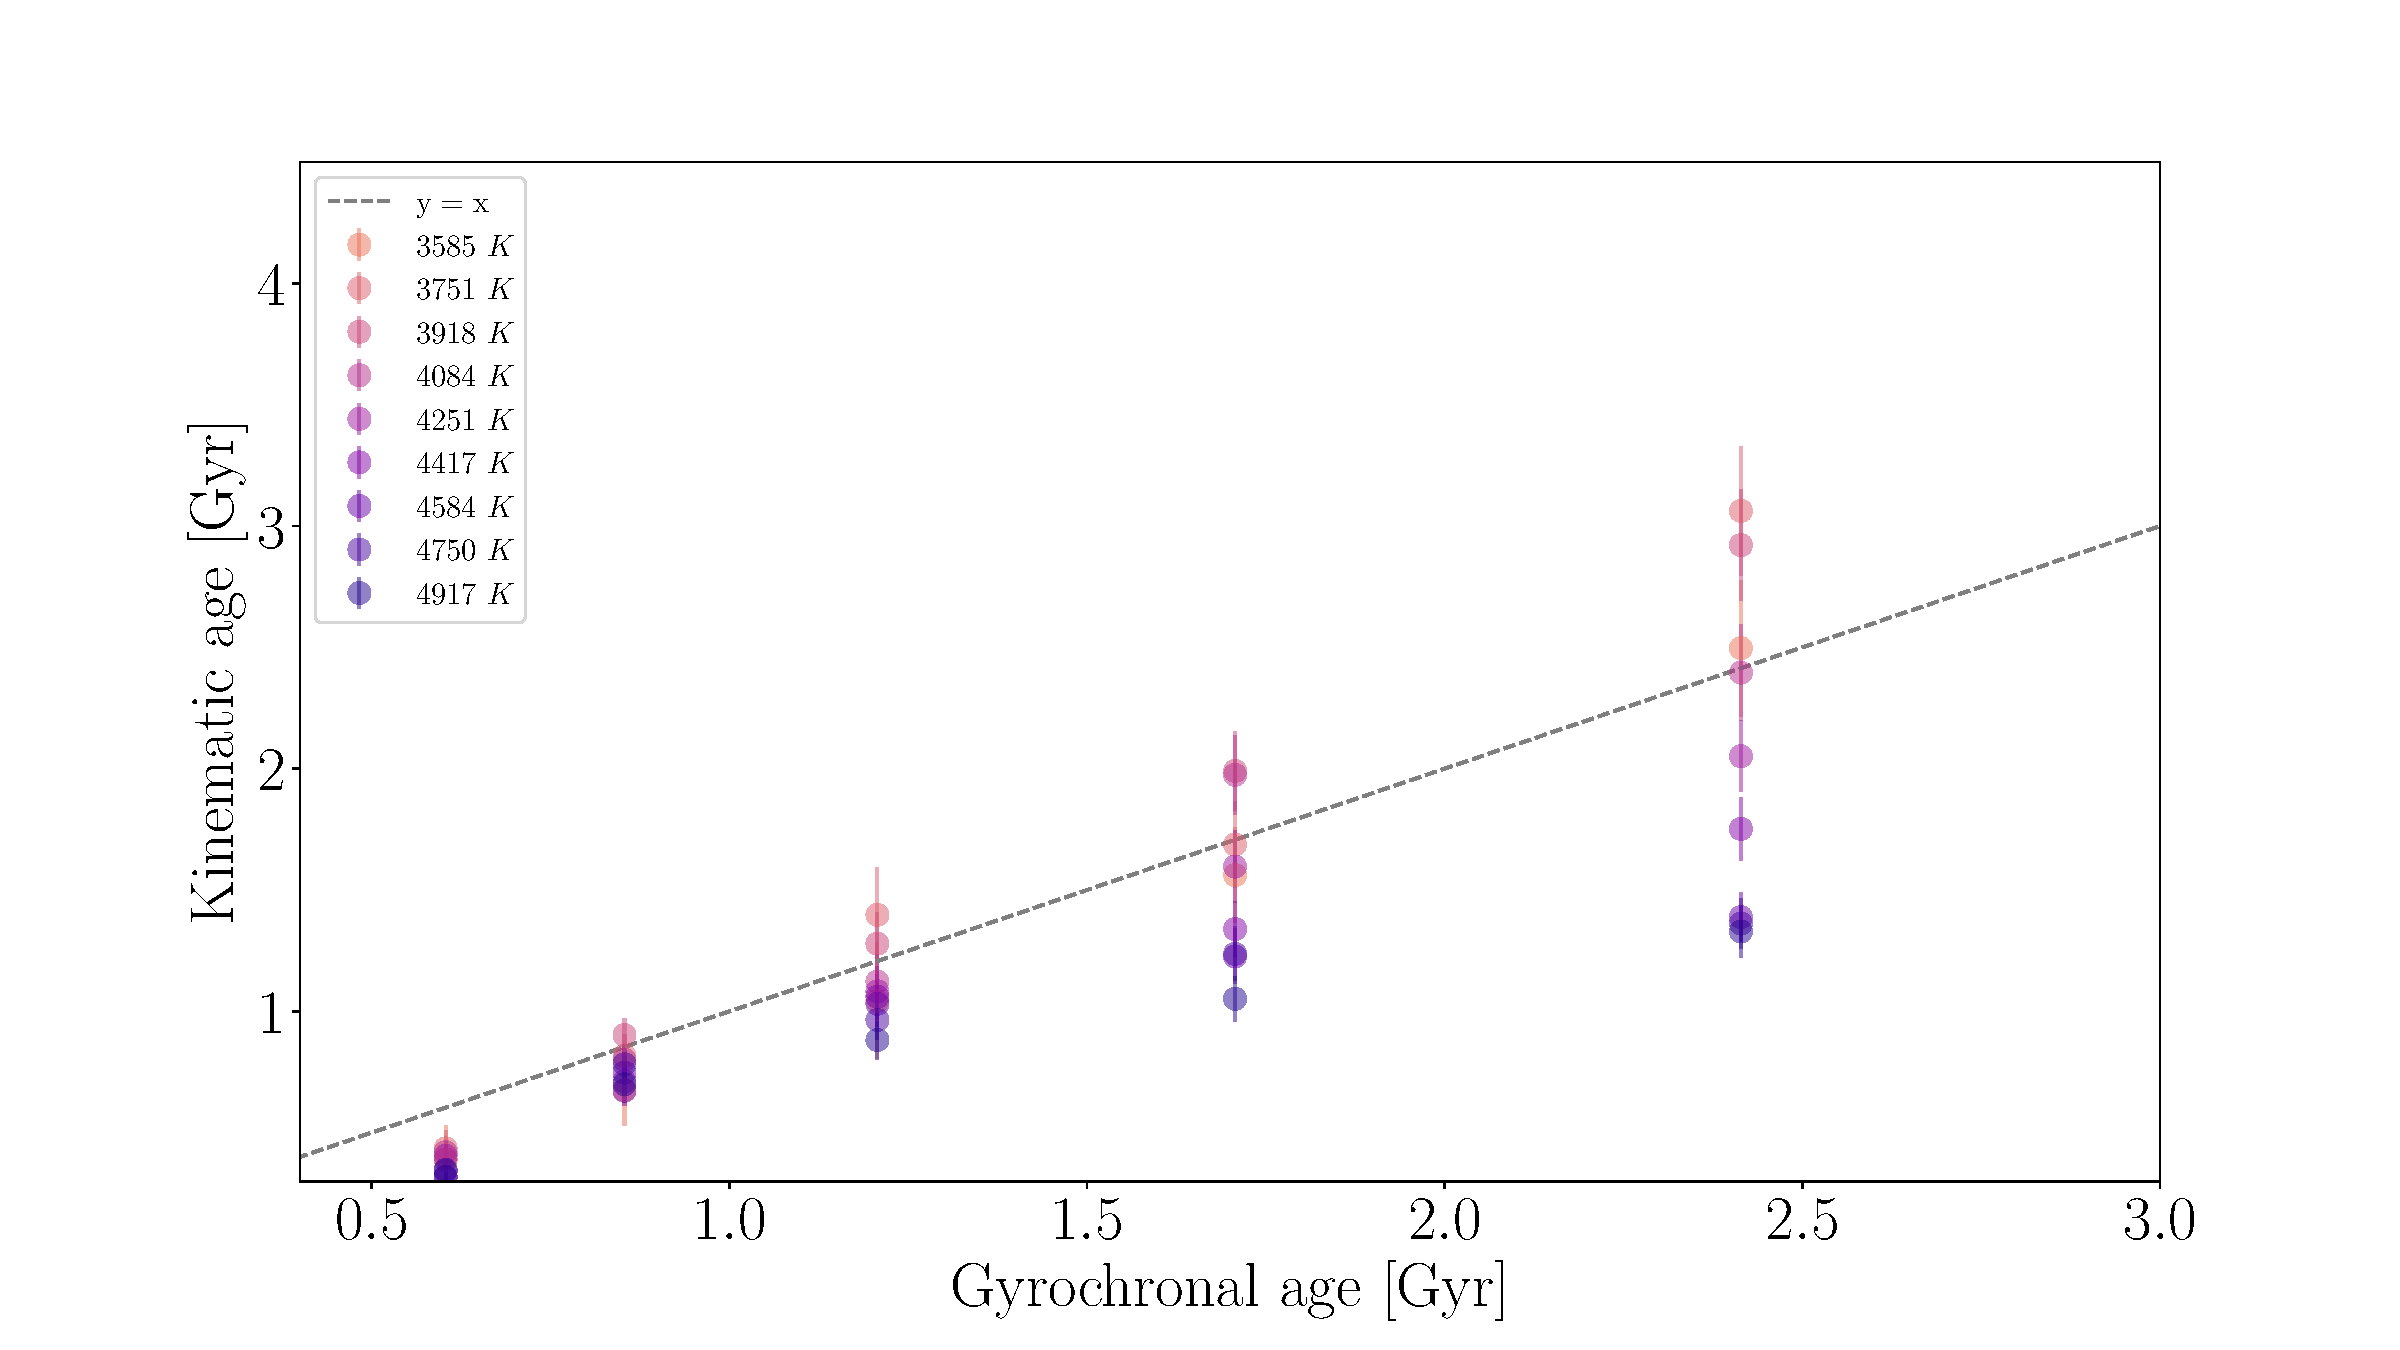
\includegraphics[width=1\textwidth]{age_comparison}
% \label{fig:age_comparison}
% \end{figure}
% Figure \ref{fig:age_comparison} shows a comparison between ages predicted by
% the \citet{holmberg2009} \vz\ AVR (using \vb\ as a proxy for \vz) and ages
% predicted by the \citet{angus2019} gyrochronology relation, for stars in
% different temperature ranges.
% The predicted kinematic ages fan out over gyrochronal time, either because the
% AVR is temperature-dependent or because the gyrochronology relations have an
% age-dependent period-color relation.
% Figure \ref{fig:age_comparion} also suggests that dynamical heating does not
% begin until after around ... Gyr:

% Alternatively, the ages of these young stars could be under-predicted by
% gyrochronology.
% These young stars have similar rotation periods to the Praesepe cluster, which
% was used to calibrate the gyrochronology relation used in this analysis.
% The ages of these young stars should, therefore, be the most accurate of the
% entire sample.
% However, they are tied to the age of the Praesepe cluster, whose age is not
% accurately known.
% \citet{angus2019} adopted an age for Praesepe of 650 Myrs, however the
% kinematic age-prediction for these stars is around 400 Myrs.
% Other studies have assigned a much older age of 800 Myrs to Praesepe
% \citep{brandt2015}.
% If the age assumed for Praesepe in the \citet{angus2019} gyrochronology
% calibration was inaccurate, the entire age {\it scale} would be incorrect.
% However, this is not what figure \ref{fig:age_comparion} shows -- it shows
% that the {\it relative} age of these youngest stars are under-predicted by
% kinematics or over-predicted by gyrochronology.

For now, we assume that the rise in velocity dispersions at cooler effective
temperatures is caused by an inaccurate period-color relation rather than
mass-dependent dynamical heating.
This assumption allows us to estimate what the shape of the period-color
relations {\it should} be.
Figure \ref{fig:age_cut} indicates that the period-color relation flattens
out, so we applied the same analysis to groups of stars with similar rotation
periods, equivalent to a completely flat period-color relation.
The top panel of figure \ref{fig:period_cut} shows the \mct\ sample with stars
in different period ranges plotted in different colors.
The bottom panel shows the velocity dispersion of each group as a function of
effective temperature.
\begin{figure}
  \caption{
This figure is similar to figure \ref{fig:age_cut}, with stars divided into
    period groups rather than age groups.
The velocity dispersion is more constant across effective temperatures for the
    most slowly rotating stars, compared to the stars selected with the
    \citet{angus2019} gyrochronology model, indicating that the gyrochronology
    models flatten out, and possibly even invert, at old ages.
}
  \centering
    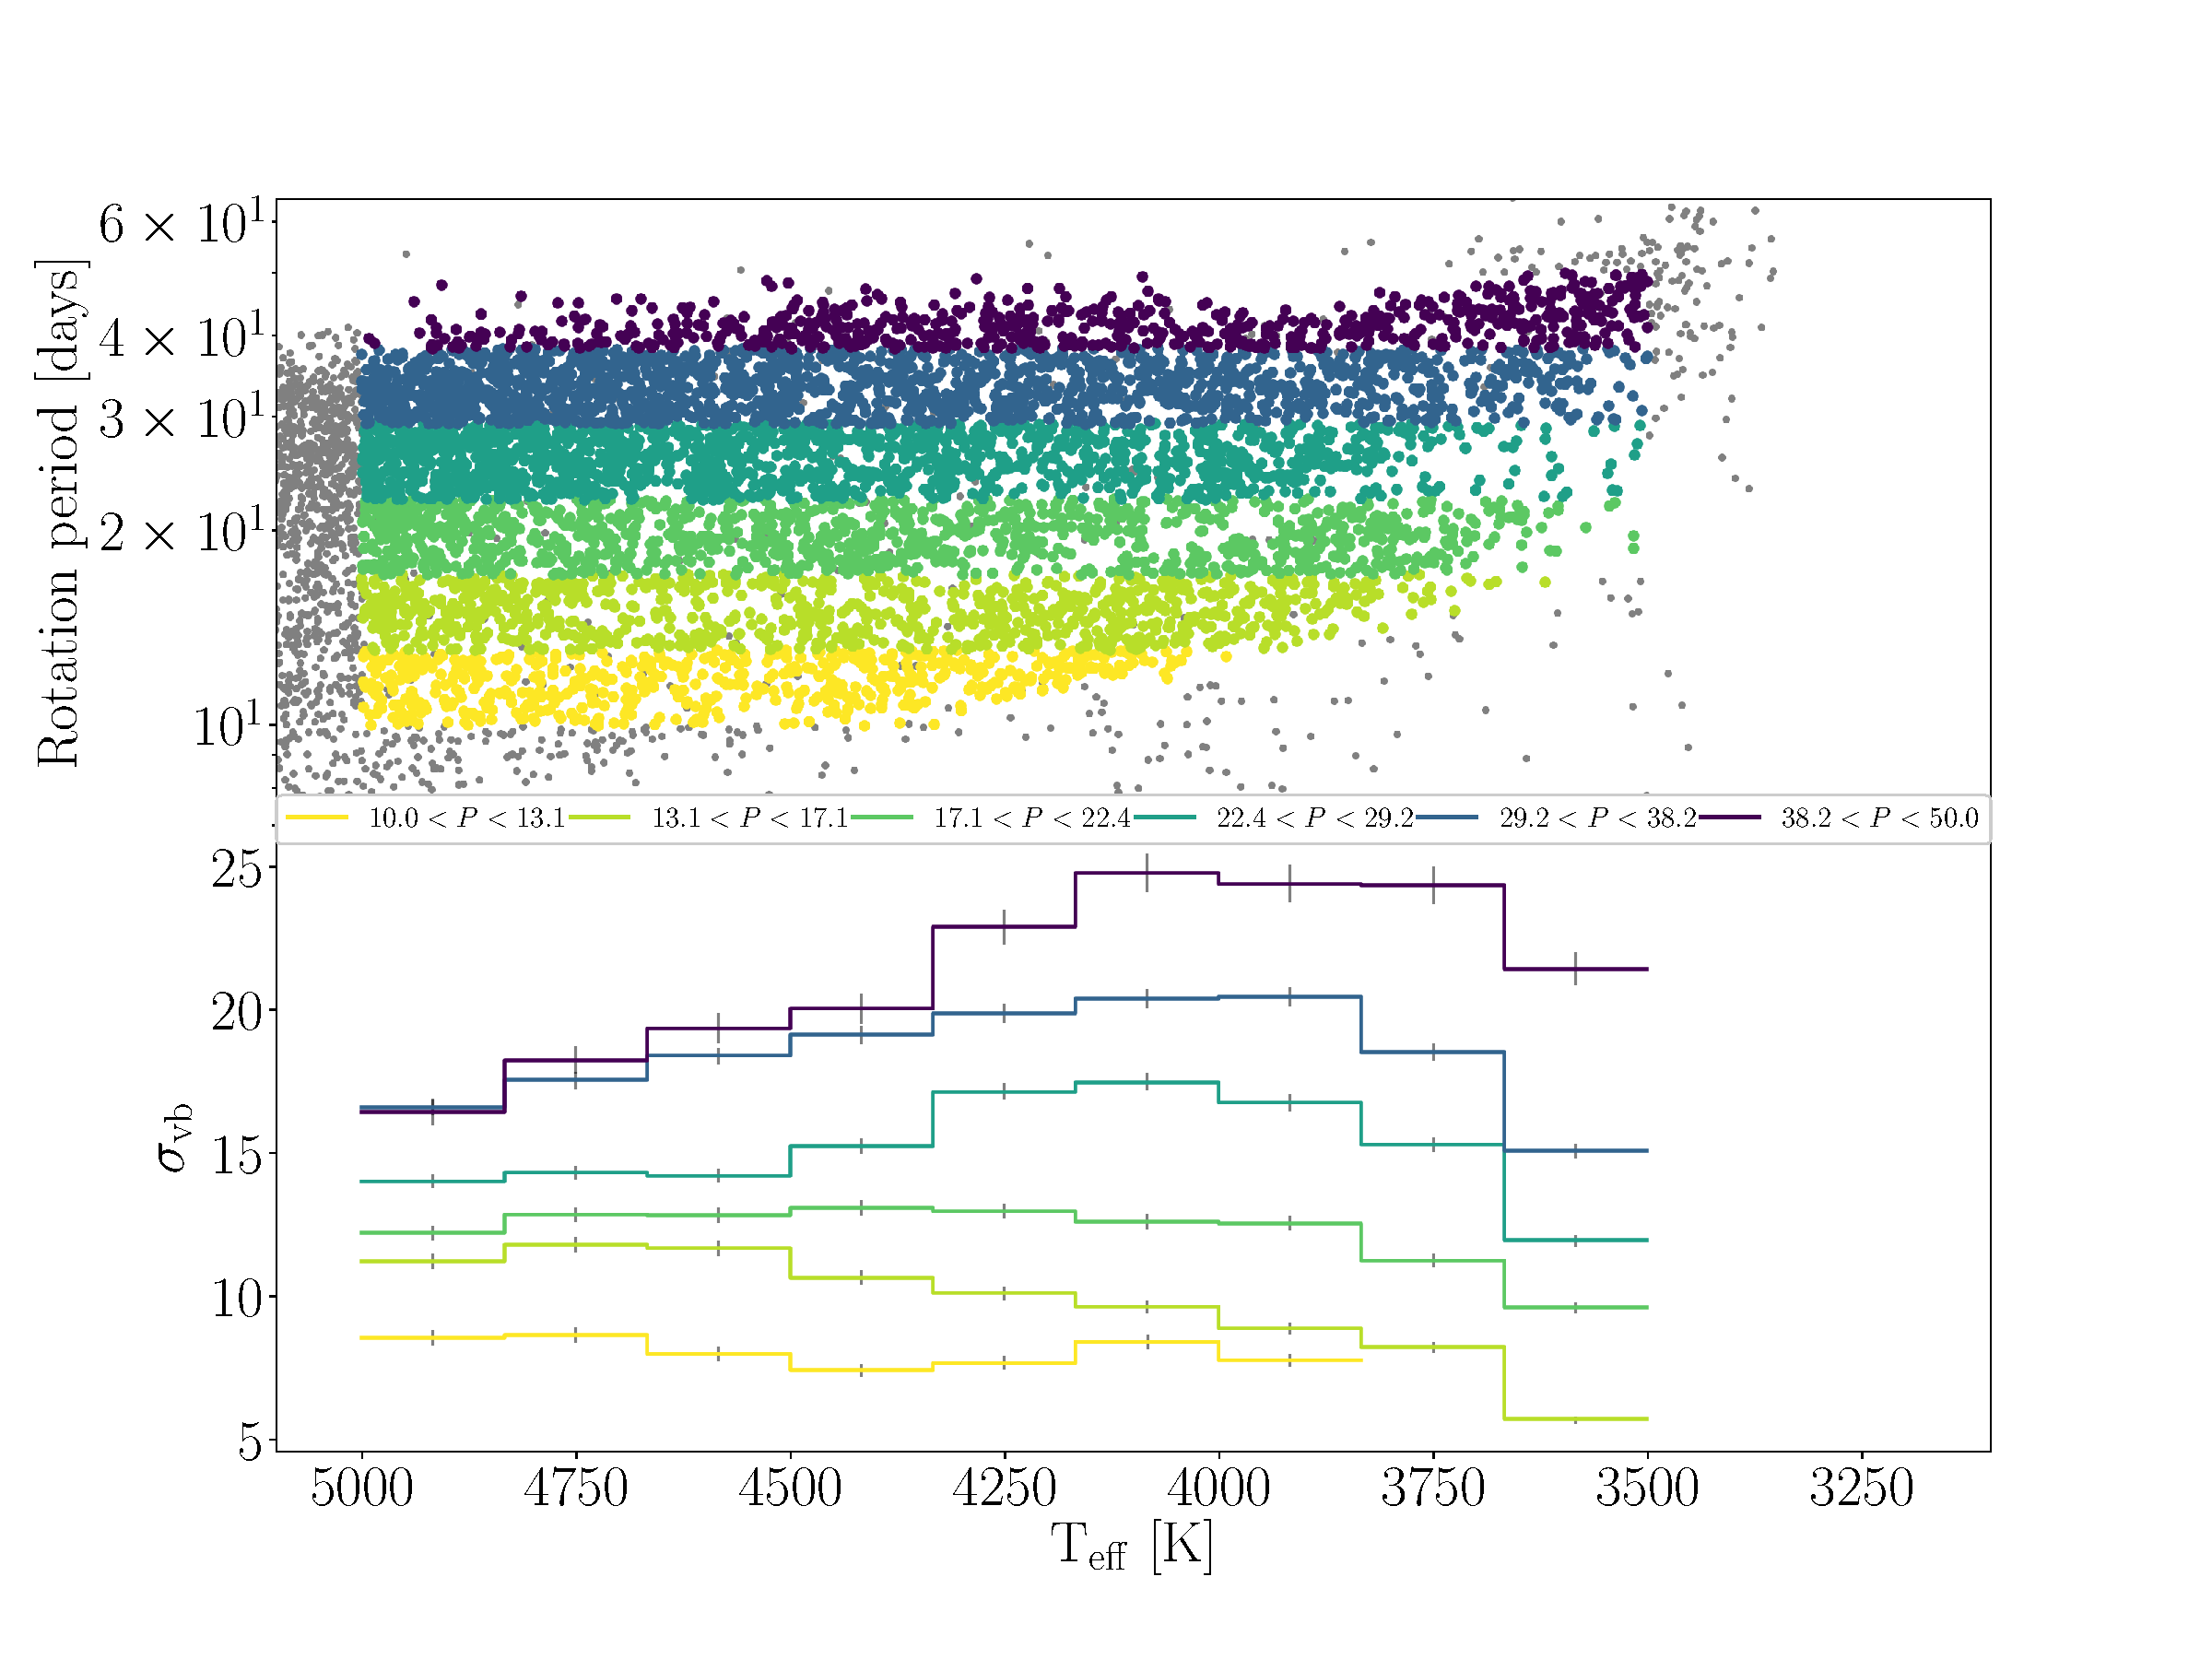
\includegraphics[width=1\textwidth]{period_cut}
\label{fig:period_cut}
\end{figure}
Once again, the velocity dispersion increases with rotation period overall.
For the most rapidly rotating groups of stars, velocity dispersion decreases
with \teff\ as expected given the positively sloped period-color relation of
Praesepe and other young clusters: late K dwarfs rotate more slowly than early
K dwarfs of the same age.
Between rotation periods of 15 and 25 days, the temperature dependence of the
velocity dispersion starts to disappear, indicating that the period-color
relation becomes flat: late K dwarfs rotate at the same rate as early K dwarfs
of the same age.
At long rotation periods, the velocity dispersion still increases with
effective temperature, although the increase is much more modest compared to
the oldest stars in figure \ref{fig:age_cut}.
This suggests that rotation period may {\it decrease} with effective
temperature, \ie\ late K dwarfs may rotate {\it more} rapidly than early K
dwarfs.
This would be a paradigm shift for gyrochronology, stellar spin-down rate is
thought to be directly tied to magnetic field strength.
The deeper convection zones of later type stars generate stronger magnetic
fields which {\it should} lead to more efficient angular momentum loss.
Unfortunately, we still cannot rule out the possibility that mass-dependent
heating is acting on these stars which could be responsible for some, if not
all, of the increased velocity dispersion at cooler effective temperatures.
